\newpage

\section{Hauptteil}\label{hauptteil}

\subsection{Google Street View im Detail}\label{street-view-detail}

Um die 360\degree\ Panoramen aufzunehmen, nutzt Google Fahrzeuge mit einer
Kamera, die durch die aufzunehmenden Straßen fahren (Siehe Abb.
\ref{fig:gsv-car}).

\begin{wrapfigure}{r}{0.4\textwidth}
  \caption{Google Street View Fahrzeug}\label{fig:gsv-car}
  \begin{center}
    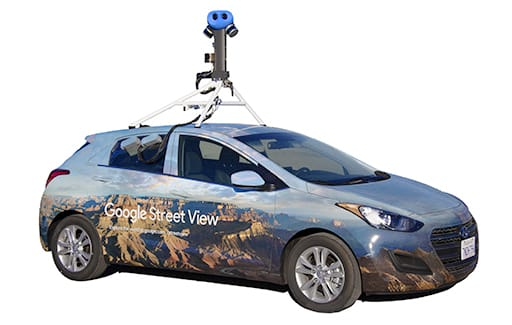
\includegraphics[width=\textwidth]{gsv-car}
    \\
    \cite[Quelle:][]{website:google-street-view:about}
  \end{center}
\end{wrapfigure}

Nachdem das Fahrzeug die Bilder aufgenommen hat, folgt die Nachbearbeitung. Hier
werden die einzelnen Bilder der Linsen in ein 360\degree\ Panorama zusammengestellt,
die Kennzeichen von anderen Fahrzeugen und die Gesichter von Personen verpixelt
und einige manuelle Nacharbeiten erledigt. Durch diesen Prozess dauert es von wenigen
Wochen bis zu mehreren Monaten, bis die aufgenommenen Bilder in Goolge Street
View der Allgemeinheit zur Verfügung gestellt werden.

Neben den Kameras haben die Street View Fahrzeuge auch noch andere Sensoren:
beispielsweise ein genaues \ac{GPS}-System, Messgeräte für Abstand, Tiefe und
Luftqualität. Zwischen 2008 und 2010 waren die Fahrzeuge auch mit einem \ac{WLAN}
Scanner ausgestattet, das die Namen und \ac{MAC} Addressen von Routern aufgezeichnet
hat, um die Positionierung in Android Smartphones zu verbessern.\footcite{website:trekview:gsv-sensors}

\subsection{Welche Daten kann man aus Google Street View erlangen}

In diesem Abschnitt wird gezeigt, wie die oben beschriebenen Daten von Google
und auch von allen anderen genutzt werden oder werden können, um einen Einblick
in die Möglichkeiten und die Implikationen für die Privatsphäre abzuschätzen.

\subsubsection{WLAN Scanning}

Durch das WLAN Scanning hat Google folgende Daten erlangen können:

\begin{enumerate}
  \item Name und MAC Addresse des WLAN Routers oder Access Points \label{name-and-mac}
  \item Stärke des WLAN Signals an der jeweiligen Position \label{signal-strength}
  \item Netzwerkverkehr von ungesicherten WLAN Netzwerken \label{network-traffic}
\end{enumerate}

Durch die Punkte \ref{name-and-mac} und \ref{signal-strength} ist es für
Google möglich, eine genauere Positionierung als GPS alleine anzubieten. Diese
Datensammlung ermöglicht Google eine Positionsbestimmung, obwohl kein GPS Signal
erfangen werden kann; besonders in dichten Städten, in denen GPS Signale häufig
durch die hohen Häuser eingeschränkt sind und viele WLANs von den Häusern
ausgehen. Der Dienst der genauren Positionsbestimung findet Anwendung in Googles
Smartphonebetriebssystem Android und der Google Maps App (unabhängig vom
Betriebssystem).

Im Gegensatz dazu steht der Punkt \ref{network-traffic}, der laut Google aus
Versehen gesammelt wurde. Die Daten würden von Google nicht genutzt werden.
Ebenso argumentiert Google, dass die Daten unvollständig sind, weil sich die
Fahrzeuge bewegen und der WLAN Channel fünfmal pro Sekunde gewechselt
wird.\footcite{website:googleblog:wifi-data-collection}

Trotzdem wurde Google für diese Datensammlung sanktioniert. Die Daten mussten in
einigen Ländern gelöscht werden\footcite{website:isec:ireland-destroy-notice}, in
Deutschland gab es am 22.04.2013 wurde ein Bußgeld in Höhe von 145 000 EUR von dem
Hamburger Datenschutzbeauftragten Johannes Caspar verhängt\footcite{website:nwzonline:google-wifi-sanction}
und in den USA wurde vom Attorney General ein Bußgeld in Höhe von 7 Mio. USD verhängt\footcite{website:connecticut:million-gsv}.

\subsubsection{Fotos}

Die Daten aus dem WLAN Scanning sind nicht für alle verfügbar. Es werde auf der
Website und der mobilen App nur die 360\degree\ Panoramen bereitgestellt. Es ist
also interessant zu sehen, welche Daten man aus diesen Bildern extrahieren kann.

Die offentsichtlichsten personenbezogenen Daten - Gesichter und Kennzeichen -
werden bereits automatisch verpixelt. Danach wird durch Google Mitarbeiter
noch einmal validiert, dass diese Merkmale wirklich verpixelt wurden. Nutzer von
Google Street View können Bilder, in denen dieser Prozess nicht funktioniert
hat, zu einer erneuten manuellen Nachbesserung melden.

In den Bildern befinden sich Informationen, die nicht alle haben sollen: Bilder
eines Einganges zu einer Basis der Britische Spezialeinheit Special Air Services
haben dazu geführt, dass das Ministery of Defense zur Löschung der Bilder
auffordert\footcite{website:bbc:herefordshire}. Ebenso ergab sich ähnliches in
den USA und deren militärischen
Basen\footcite{website:reuters:pentagon-takedown-notice}.

Wissenschaftler:innen nutzen Google Street View als Datengrundlage für eine
weitreichende Datenanalyse im Bereich Big Data und Machine Learning. Folgende
Themen und Werke werden als Beispiele näher beschrieben:

\begin{enumerate}
  \item Zur Planung von 5G Masten - \cite{Zhang_2020}\label{5g}
  \item Das Volumen an Fußgängern - \cite{YIN2015337}\label{pedestrian-volume}
  \item Die Demographie der Nachbarschaft - \cite{Gebru13108}\label{demographics}
  \item Die Wahrscheinlichkeit für einen Autounfall eines Bewohners - \cite{kita2019google}\label{car-accident}
  \item Die Gesundheit von Bewohnern einer bestimmten
  Nachbarschaft - \cite{8933431} und \cite{DBLP:journals/corr/abs-1905-06464}\label{health}
\end{enumerate}

In Arbeit \ref{5g} werden die Bilder von Google Street View genutzt, um
herauszufinden, wo sich Straßenbeleuchtungsmasten befinden. Es wird dadurch
möglich, Masten für den neuen Funkstandard 5G zu planen, weil diese relativ
günstig an vorhandener Straßenbeleuchtung angebracht werden können.

Arbeit \ref{pedestrian-volume} misst das Volumen an Fußgängern, die zu der
Aufnahme der Google Street View Bilder draußen waren. Diese Daten können
genutzt werden, um zu urteilen, wie aktiv Personen in einer Umgebung sind und
was Personen dazu bringt, mehr Zeit draußen zu verbringen. Weitere Informationen
über den Zusammenhang von Stadtbild und physikalischer Aktivität findet man in
den Forschungsarbeiten von Li Yin an der State University of New York.

In Punkt \ref{demographics} wird gezeigt, dass Google Street View ebenso genutzt
werden kann, um Aussagen über die Nachbarschaft oder Region zu treffen. In
dieser Arbeit werden die fotografierten Autos (Marke, Modell und Jahr) als
Grundlage für die Analyse der Demographie genutzt. Es konnten Einkommen,
Hautfarbe, Bildung und politische Ausrichtung aufgrund dieser Daten bestimmt
werden.

Die Arbeit \ref{car-accident} beschreibt, wie Bilder von Google Street View
besseren Aufschluss über die Wahrscheinlichkeit eines Autounfalls geben kann,
als andere von Versicherungen genutzten Risikomodelle. Diese Daten,
argumentieren die Autoren, können später auch von den Banken genutzt werden, da
in anderen Arbeiten gezeigt wurde, dass Kreditwürdigkeit und Risikobewertung von
Versicherungen zusammenhängen\footcite{doi:10.1080/10920277.2016.1209118}.

In Arbeit \ref{health} ist zu sehen, dass die Bilder, die aus Google Street View
einzusehen sind, auch dafür genutzt werden können, um Aussagen über die
Gesundheit der Bewohner zu treffen. Solche Daten sind für Stadplaner
interessant, die überprüfen können, ob was an der Umgebung geändern werden kann,
um Bewohner zu mehr Bewegung anzuregen. Ebenfalls sind die Daten für
Krankenversicherungen interessant, um das Risiko von Krankheiten genauer
abzuschätzen.

\subsection{Ein Pro und Contra zu Google Street View}

In diesem Unterkapitel werden die zuvor genannten Informationen
zusammengetragen, um Argumente für und gegen Google Street View zu bilden.

Grundsätzlich macht Google mit den Bildern nur einen Prozess einfacher: Anstatt
selbst die Straßen entlangzufahren, kann man einfach die Bilder von Google
Street View bekommen. Einerseits können Forscher:innen die Daten nutzen, um
einen guten Beitrag zu leisten; andererseits erleichtert es Menschen mit
schlechten Absichten, die Daten für andere Zwecke zu missbrauchen.

% \begin{listing}
%   \item Soll Deutschland oder die EU von Google Stret View ausgeschlossen werden?
%   \item Soll nur die Neuaufnahme von Bildern verboten werden?
%   \item Dürfen die Google Street View Autos noch immer Daten für Google intern sammeln?
%   \item Soll Google Street View in Deutschland erweitert werden?
% \end{listing}


\subsubsection{Positiver Nutzen von Google Street View}

Wie in Unterkapitel \ref{street-view-detail} beschrieben, werden Daten über
Luftqualität von Google gesammelt. Diese Daten können von Klimaforscher:innen,
Stadtplanern und Regierungen genutzt werden, um den akteuellen Stand zum
Klimawandel zu überprüfen. Diese Daten helfen der Menschheit dabei, effektiv
gegen den Klimawandel vorzugehen und zukünftige Stadtprojekte nachhaltig zu
planen.

Auch der ursprüngliche Zweck von Google Street View ist generell als positiv zu
bewerten. Es ist bei Autofahrten möglich die Route durch ein komplexes
Straßensystem schon vor Antritt der Reise zu planen. Es ist möglich, sich
markante Merkmale herauszusuchen, die während der Fahrt leicht zu erkennen sind.
Dafür müssen die Bilder von Google Street View aber aktuell sein. Aktuelle
Aufnahmen sind hierzu notwendig; Fotos deutscher Straßen sind allerdings
veraltet und die Abdeckung ist gering.

Google zeigt durch eine Fallstudie, dass lokale Unternehmen von Google Street
View und virtuellen Touren
profitieren\footcite{website:google:impact-for-local-businesses}. Personen gehen
lieber an Orte, die einfach zu finden sind und von denen sie im vorhinein sehen
können, was sie erwartet. Dies gilt sowohl für lokale Unternehmen als auch für
den Tourismus einer Region oder eines Landes. Eine weitere Einschränkung von
Google Street View würde dem Tourismus schaden, eine größere Abdeckung von
Google Street View würde sich positiv auf den Tourismus auswirken. Durch Google
Street View kann sich ein besserer Überblick über Sehenswürdigkeiten verschafft
werden, als es bei anderen Arten der Bildbetrachtung möglich ist. Dies erhöht
die Attraktivität und Zugänglichkeit von Regionen.

Zuletzt ist es möglich, die eigene Hausfront verpixeln zu lassen. Dieser Opt-Out
kann verhindern, dass bestimmte personenbezogene Daten ermittelt werden können.
Besonders die Kategorisierung des Hauses (Anzahl Fenster, Garage vorhanden,
Zustand des Hauses) oder des Autos (Marke, Modell) kann dadurch verhindert
werden. Genau diese Daten hatten es in den oben beschriebenen Arbeiten
ermöglicht, Aussagen über Einkommen, Kreditwürdigkeit und politische Ausrichtung
zu treffen.

\subsubsection{Negative Seiteneffekte von Google Street View}

Wie aus den vorangegangenen Arbeiten deutlich wurde, ist das automatische
Verpixeln häufig nicht gut genug, um alle Daten zu anonymisieren. Häuserfronten
und Autos der Bewohner:innen bleiben ersichtlich; ebenso können Personen an
Körperbau und Kleidung erkannt werden. Dies ist besonders dann ein Problem, wenn
Personen bei Tätigkeiten fotografiert werden, die vom Umfeld der Person als
negativ wahrgenommen werden kann; etwa der Besuch eines Strip Clubs.

Auch kann das Verpixeln einer Hausfassade so interpretiert werden, dass dort
ansässige Personen etwas zu verstecken hätten. Unternehmen können Bewohner:innen
von verpixelten Häusern diskriminieren, indem Sie Rabatte oder Vorteile für
Bewohner:innen von nicht verpixelten Häusern anbieten.

Ein häufiges Argument ist die Erleichterung der Planung von Einbrüchen oder
Überfällen. So sollen lohnende Gebäude leichter gefunden und potenzielle
Eintrittspunkte besser identifiziert werden können.  Bei der Entfernung von
Bildern militärischer Basen wurde argumentiert, dass Terroristen somit ihr
nächstes Ziel auskundschaften können.

\subsection{Die Realität und Machbarkeit einer Einschränkung von Google Street View}

Laut deutschem Recht darf jeder Bilder von öffentlichen Straßen machen und
veröffentlichen - auch Google. Nach dem KunstUrhG §23 dürfen Bilder von Personen
veröffentlich werden, wenn diese nur ein Beiwerk sind. Google stellt sogar durch
die Verpixelung sicher, dass Personen schwieriger bis gar nicht mehr
identifizierbar sind.

Ebenso sind Argumente, dass die Kamera in einer Höhe von 3 Metern montiert ist
und somit Einblick über Gartenzäune bekommen kann, vor Gericht entkräftet
worden\footnote{LG Berlin, Urteil vom 13.09.2010 - 37 O 363/10}.

Laut aktuellem Recht ist Google Street View vom Gesetz und Gericht bestätigt
worden. Es bleibt zuletzt die Frage, ob das Gesetz angepasst werden muss, um die
Freiheit von Personen und ihren Daten auch in der aktuellen digitalen Zeit zu
schützen. Diese Frage wird in Fazit noch einmal aufgegriffen.
